
\documentclass{llncs} 

\usepackage{algorithm}
\usepackage{algpseudocode}
\usepackage{graphicx}


\title{Investigating Exploration Techniques in Anytime Heuristic Search}
\author{Dawson Brown (500780579)\\dawson.brown@ryerson.ca}
\institute{Ryerson University}

\date{}
\begin{document}
\maketitle
\pagestyle{plain}

\begin{abstract}
    hello
\end{abstract}


\section{Introduction}

Evaluation Metrics:
\begin{enumerate}
    \item Total Stored nodes \cite{hansen2007anytime}
    \item Total Expanded nodes \cite{hansen2007anytime}
    \item Solution quality at fixed CPU intervals \cite{thayer2012better}
    \item Average time between solutions \cite{thayer2012better}
    \item Average number of solutions found before optimal solution was found
    \item Average time taken to find optimal solution
    \item Lower bound on optimal solution at fixed CPU intervals
\end{enumerate}


Parameters:
\begin{enumerate}
    \item Weights: 1.3, 1.5, 2 \cite{hansen2007anytime} (1.3 performed best, so maybe just do that?)
    \item Epsilon: 0.1, 0.2, 0.3 \cite{valenzano2014comparison}
    \item Unit cost and inverse cost
\end{enumerate}


\section{Background}



\section{Exploration in AWA$^*$}

\subsection{$\epsilon$-AWA$^*$}


\subsection{$\alpha \beta$-AWA$^*$}

\noindent
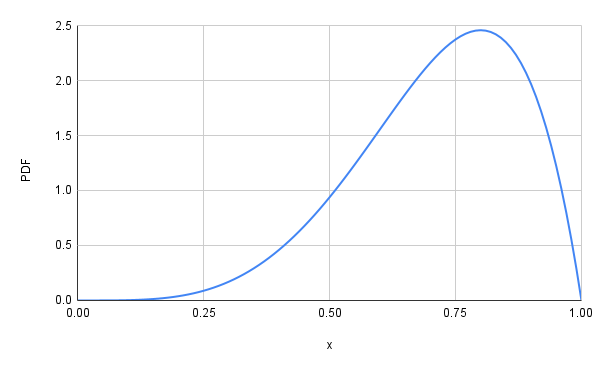
\includegraphics[scale=0.4]{media/chart.png}



\section{Evaluation}
In order to evaluate the usefulness of exploration in AWA$^*$ a number of experiments were conducted on 2 problem domains--the unit-cost and the inverse-cost sliding tile puzzles. In each domain, multiple weights and epsilon values will be used to parameterize the three algorithms. For the weights, 1.3, 2, and 5, will be used in order to see how weighing the heuristic more or less impacts the search. For $\epsilon-$AWA$^*$ and $\alpha \beta-$AWA$^*$, 0.1 and 0.3 will be used as the $\epsilon$ value in order to see how more or less random exploration impacts the search. 

Degraded heuristic.

Summarize architecture.

\subsection{Unit-Cost Tile Puzzle}

\subsubsection{Degraded Heuristic}


\subsection{Inverse-Cost Tile Puzzle}


\subsubsection{Degraded Heuristic}


\section{Conclusion}


\begin{algorithm}
\caption{$\epsilon-AWA^*$ node selection}\label{alg:eawa}
\begin{algorithmic}
\State $y \gets $ randrange(0,1)
\If{$y \leq epsilon$}
    \State\Return randomSample($OPEN$)
\Else{}
    \State\Return $\arg \min_{x \in OPEN} f'(x)$
\EndIf
\end{algorithmic}
\end{algorithm}


\begin{algorithm}
\caption{$\alpha \beta-AWA^*$ node selection}\label{alg:abawa}
\begin{algorithmic}
\Require $\gamma \gets beta(\alpha, \beta)$
\State $y \gets $ randrange(0,1)
\If{$y \leq epsilon$}
    \State $row \gets $ sampleRow($OPEN$, $\gamma$)
    \State $start \gets 2^{row}-1$
    \State $end \gets 2 \cdot start$
    \State \Return randomSample($OPEN[start:end]$)
\Else{}
    \State \Return $\arg \min_{x \in OPEN} f'(x)$
\EndIf
\end{algorithmic}
\end{algorithm}


\newpage
\bibliography{ref}
\bibliographystyle{splncs04}

\end{document}